% !TEX encoding = UTF-8
% !TEX TS-program = pdflatex
% !TEX root = ../tesi.tex

%**************************************************************
\chapter{Analisi dei requisiti}
\label{cap:analisi-requisiti}
%**************************************************************

\intro{In questo capitolo verranno elencati i casi d'uso delle funzionalità implementate con i relativi requisiti ed i loro tracciamento}\\

\section{Casi d'uso}
\label{sec:casi-uso}

Per lo studio dei casi d'uso del prodotto creato sono stati creati dei diagrammi.
Questi diagrammi, detti appunto dei casi d'uso (in inglese \emph{Use Case Diagram}), sono diagrammi di tipo \gls{uml} dedicati alla descrizione del sistema e delle funzioni o servizi offerti da un esso, e come gli utilizzatori interagiscono con esso.\\
Lo strumento utilizzato per la realizzazione di tali diagrammi è draw.io, piattaforma online che permette di creare diagrammi direttamente nel browser e salvarli nel proprio cloud di Google.

\subsection{Attori dei casi d'uso}
\label{subsec:attori}

Dopo un'attenta analisi ho concluso che per le funzionalità offerte sono presenti unicamente attori primari, in quanto non ci sono collegamenti con alcun \gls{frameworkg} o libreria esterna.
Di conseguenza i possibili attori dei casi d'uso analizzati sono i seguenti attori primari:
\begin{itemize}
	\item \textbf{utente non autenticato}: indica che l'utente non ha ancora effettuato l'autenticazione o la registrazione all'interno della web application;
	\item \textbf{utente autenticato}: indica che l'utente ha effettuato l'autenticazione all'interno della web application e comporta che può accedere a diverse funzionalità che sarebbero altrimenti inaccessibili.
\end{itemize}

\begin{figure}[H] 
	\centering 
	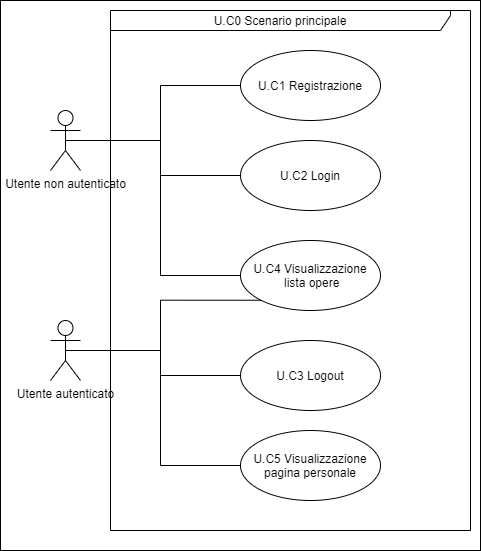
\includegraphics[width=0.8\columnwidth]{usecase/uc0} 
	\caption{U.C0 Scenario principale}
\end{figure}

\newpage

\begin{usecase}{1}{Registrazione}\label{uc1}
	\begin{figure}[H] 
		\centering 
		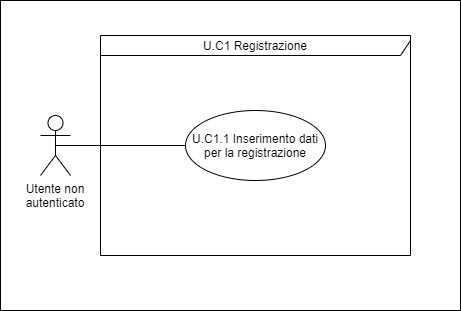
\includegraphics[width=0.7\columnwidth]{usecase/UC1} 
		\caption{U.C1 Registrazione}
	\end{figure}
\usecaseactors{Utente non autenticato.}
\usecasepre{L'utente non è ancora presente nei registri del sistema.}
\usecasedesc{L'utente accede all'applicazione e naviga fino alla pagina di registrazione. L'utente inserisce i dati necessari e li conferma, questo porta l'utente a possedere un account nel sistema.}
\usecasepost{L'utente risulta presente nei registri del sistema ed è autenticato nella piattaforma.}
\end{usecase}

\begin{usecase}{1.1}{Inserimento dati per la registrazione}\label{uc1.1}
	\begin{figure}[H] 
		\centering 
		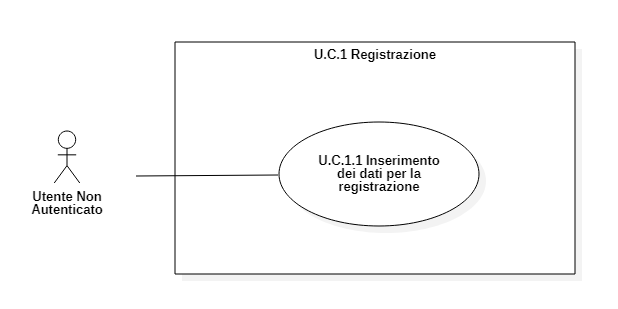
\includegraphics[width=0.9\columnwidth]{usecase/UC1.1} 
		\caption{U.C1.1 Inserimento dei dati per la registrazione}
	\end{figure}
\usecaseactors{Utente non autenticato.}
\usecasepre{L'utente non autenticato si trova nella pagina di registrazione.}
\usecasedesc{L'utente non autenticato compila i campi nel seguente modo:
\begin{itemize}
	\item Inserimento del nome (\ref{uc1.1.1});
	\item Inserimento del cognome (\ref{uc1.1.2});
	\item Inserimento dell'email (\ref{uc1.1.3});
	\item Inserimento della password (\ref{uc1.1.4});
	\item Inserimento della conferma della password (\ref{uc1.1.5});
	\item Inserimento dell'anno di nascita (\ref{uc1.1.6});
	\item Inserimento del Wallet Address (\ref{uc1.1.7}).
\end{itemize}
}
\usecasepost{L'utente ha completato la compilazione dei campi e può procedere con la registrazione.}
\end{usecase}

\begin{usecase}{1.1.1}{Inserimento del nome}\label{uc1.1.1}
\usecaseactors{Utente non autenticato.}
\usecasepre{L'utente non è autenticato e non ha compilato questo campo.}
\usecasedesc{L'utente non autenticato inserisce il proprio nome.}
\usecaseest{Viene effettuato un controllo e risulta che questo campo non è stato compilato quindi si presenta un messaggio di errore e viene fornita la possibilità di inserire nuovamente il dato (\ref{uc6}).}
\usecasepost{L'utente ha inserito il nome.}
\usecaseest{L'utente non inserisce nulla e appare il messaggio di errore.}
\end{usecase}

\begin{usecase}{1.1.2}{Inserimento del cognome}\label{uc1.1.2}
\usecaseactors{Utente non autenticato.}
\usecasepre{L'utente non è autenticato e non ha compilato questo campo.}
\usecasedesc{L'utente non autenticato inserisce il proprio cognome.}
\usecaseest{Viene effettuato un controllo e risulta che questo campo non è stato compilato quindi si presenta un messaggio di errore e viene fornita la possibilità di inserire nuovamente il dato (\ref{uc6}).}
\usecasepost{L'utente ha inserito il cognome.}
\end{usecase}

\begin{usecase}{1.1.3}{Inserimento dell'email}\label{uc1.1.3}
\usecaseactors{Utente non autenticato.}
\usecasepre{L'utente non è autenticato e non ha compilato questo campo.}
\usecasedesc{L'utente non autenticato inserisce la sua email.}
\usecaseest{
	\begin{itemize}
		\item Viene effettuato un controllo e risulta che questo campo non è stato compilato quindi si presenta un messaggio di errore e viene fornita la possibilità di inserire nuovamente il dato (\ref{uc6});
		\item Viene effettuato un controllo sul campo inserito e risulta non essere valido quindi si presenta un messaggio di errore e viene fornita la possibilità di inserire nuovamente il dato (\ref{uc7}).
	\end{itemize}
}
\usecasepost{L'utente ha inserito l'email.}
\end{usecase}

\begin{usecase}{1.1.4}{Inserimento della password}\label{uc1.1.4}
\usecaseactors{Utente non autenticato.}
\usecasepre{L'utente non è autenticato e non ha compilato questo campo.}
\usecasedesc{L'utente non autenticato inserisce la sua password.}
\usecaseest{
	\begin{itemize}
		\item Viene effettuato un controllo e risulta che questo campo non è stato compilato quindi si presenta un messaggio di errore e viene fornita la possibilità di inserire nuovamente il dato (\ref{uc6});
		\item Viene effettuato un controllo sul campo inserito e risulta non essere valido quindi si presenta un messaggio di errore e viene fornita la possibilità di inserire nuovamente il dato (\ref{uc7}).
	\end{itemize}
}
\usecasepost{L'utente ha inserito la password.}
\end{usecase}

\begin{usecase}{1.1.5}{Inserimento della conferma della password}\label{uc1.1.5}
\usecaseactors{Utente non autenticato.}
\usecasepre{L'utente non è autenticato e non ha compilato questo campo.}
\usecasedesc{L'utente non autenticato inserisce la conferma della password.}
\usecaseest{
	\begin{itemize}
		\item Viene effettuato un controllo e risulta che questo campo non è stato compilato quindi si presenta un messaggio di errore e viene fornita la possibilità di inserire nuovamente il dato (\ref{uc6});
		\item Viene effettuato un controllo sul campo inserito e risulta non essere valido quindi si presenta un messaggio di errore e viene fornita la possibilità di inserire nuovamente il dato (\ref{uc8});
		\item Viene effettuato un controllo di uguaglianza con la password precedentemente inserita e i due campi non risultano uguali quindi si presenta un messaggio di errore e viene fornita la possibilità di inserire nuovamente il dato(\ref{uc9}).
	\end{itemize}
}
\usecasepost{L'utente ha inserito la conferma della password.}
\end{usecase}

\begin{usecase}{1.1.6}{Inserimento dell'anno di nascita}\label{uc1.1.6}
\usecaseactors{Utente non autenticato.}
\usecasepre{L'utente non è autenticato e non ha compilato questo campo.}
\usecasedesc{L'utente non autenticato inserisce il proprio anno di nascita.}
\usecaseest{
	\begin{itemize}
		\item Viene effettuato un controllo e risulta che questo campo non è stato compilato quindi si presenta un messaggio di errore e viene fornita la possibilità di inserire nuovamente il dato (\ref{uc6});
		\item Viene effettuato un controllo sul campo inserito e risulta non essere valido in quanto l'utente risulta essere non maggiorenne quindi si presenta un messaggio di errore e viene fornita la possibilità di inserire nuovamente il dato (\ref{10}).
	\end{itemize}
}
\usecasepost{L'utente ha inserito l'anno di nascita.}
\end{usecase}

\begin{usecase}{1.1.7}{Inserimento del Wallet Address}\label{uc1.1.7}
\usecaseactors{Utente non autenticato.}
\usecasepre{L'utente non è autenticato e non ha compilato questo campo.}
\usecasedesc{L'utente non autenticato inserisce il Wallet Address.}
\usecaseest{
	\begin{itemize}
		\item Viene effettuato un controllo e risulta che questo campo non è stato compilato quindi si presenta un messaggio di errore e viene fornita la possibilità di inserire nuovamente il dato (\ref{uc6});
		\item Viene effettuato un controllo sul campo inserito e risulta non essere valido quindi si presenta un messaggio di errore e viene fornita la possibilità di inserire nuovamente il dato (\ref{11}).
	\end{itemize}
}
\usecasepost{L'utente ha inserito il Wallet Address.}
\end{usecase}

\begin{usecase}{2}{Login}\label{uc2}
	\begin{figure}[H] 
		\centering 
		\includegraphics[width=0.8\columnwidth]{usecase/UC2} 
		\caption{U.C2 Login}
	\end{figure}
\usecaseactors{Utente non autenticato.}
\usecasepre{L'utente non è autenticato ma è presente nei registri di sistema.}
\usecasedesc{L'utente accede all'applicazione e naviga fino alla pagina di login. L'utente inserisce i dati necessari (\ref{uc2.1}) e li conferma, questo porta l'utente ad autenticarsi nel sistema.}
\usecaseest{L'utente inserisce i dati ma non è presente nel database quindi si presenta un messaggio di errore e viene fornita la possibilità di inserire nuovamente i dati (\ref{uc12}).}
\usecasepost{L'utente risulta autenticato nella piattaforma.}
\end{usecase}

\begin{usecase}{2.1}{Inserimento dati per il login}\label{uc2.1}
	\begin{figure}[H] 
		\centering 
		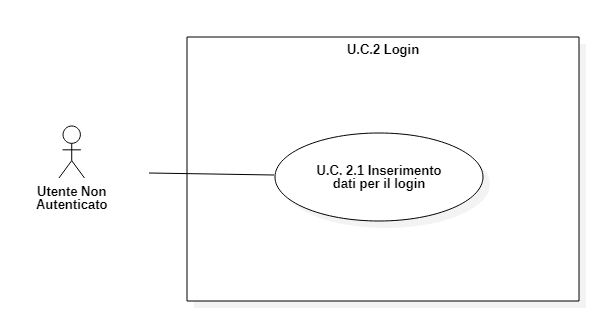
\includegraphics[width=0.8\columnwidth]{usecase/UC2.1} 
		\caption{U.C2.1 Inserimento dati per il login}
	\end{figure}
\usecaseactors{Utente non autenticato.}
\usecasepre{L'utente non autenticato si trova nella pagina di login.}
\usecasedesc{L'utente non autenticato compila i campi nel seguente modo:
\begin{itemize}
	\item Inserimento della email (\ref{uc2.1.1});
	\item Inserimento della password (\ref{uc2.1.2}).
\end{itemize}}
\usecasepost{L'utente è autenticato come utente autenticato all'interno della web application.}
\end{usecase}

\begin{usecase}{2.1.1}{Inserimento della email}\label{uc2.1.1}
\usecaseactors{Utente non autenticato.}
\usecasepre{L'utente non autenticato si trova nella pagina di login e possiede le credenziali di accesso.}
\usecasedesc{L'utente, per procedere con l'autenticazione inserisce l'email.}
\usecaseest{
	\begin{itemize}
		\item Viene effettuato un controllo e risulta che questo campo non è stato compilato quindi si presenta un messaggio di errore e viene fornita la possibilità di inserire nuovamente il dato (\ref{uc6});
		\item Viene effettuato un controllo sul campo inserito e risulta non essere valido quindi si presenta un messaggio di errore e viene fornita la possibilità di inserire nuovamente il dato (\ref{uc7}).
	\end{itemize}}
\usecasepost{L'utente ha inserito l'email.}
\end{usecase}

\begin{usecase}{2.1.2}{Inserimento della password}\label{uc2.1.2}
	\usecaseactors{Utente non autenticato.}
	\usecasepre{L'utente non autenticato si trova nella pagina di login e possiede le credenziali di accesso.}
	\usecasedesc{L'utente, per procedere con l'autenticazione inserisce la password.}
	\usecaseest{
		\begin{itemize}
			\item Viene effettuato un controllo e risulta che questo campo non è stato compilato quindi si presenta un messaggio di errore e viene fornita la possibilità di inserire nuovamente il dato (\ref{uc6});
			\item Viene effettuato un controllo sul campo inserito e risulta non essere valido quindi si presenta un messaggio di errore e viene fornita la possibilità di inserire nuovamente il dato (\ref{uc8}).
		\end{itemize}}
	\usecasepost{L'utente ha inserito la password.}
\end{usecase}

\begin{usecase}{3}{Logout}\label{uc3}
	\usecaseactors{Utente autenticato.}
	\usecasepre{L'utente è autenticato e vuole uscire dal proprio account.}
	\usecasedesc{L'utente vuole uscire dal proprio account}
	\usecasepost{L'utente non è più autenticato}
\end{usecase}

\begin{usecase}{4}{Visualizzazione lista opere}\label{uc4}
	\begin{figure}[H] 
		\centering 
		\includegraphics[width=0.8\columnwidth]{usecase/UC4} 
		\caption{U.C4 Visualizzazione lista opere}
	\end{figure}
	\usecaseactors{Utente non autenticato.}
	\usecasepre{L'utente ha aperto il sito e si trova nella pagina iniziale.}
	\usecasedesc{L'utente può visualizzare la lista delle opere in vendita. In particolare l'utente può filtrare le opere (\ref{uc4.1}) oppure visualizzare nel dettaglio un'opera selezionata (\ref{uc4.2})}
	\usecasepost{L'utente ha visualizzato la lista.}
\end{usecase}

\begin{usecase}{4.1}{Inserimento filtro sulla lista opere}\label{uc4.1}
	\usecaseactors{Utente non autenticato.}
	\usecasepre{L'utente si trova nella pagina principale e sta visualizzando le opere.}
	\usecasedesc{L'utente può applicare dei filtri alla lista di opere presenti nella homepage.}
	\usecasepost{L'utente ha visualizzato la lista di opere filtrate.}
\end{usecase}

\begin{usecase}{4.1.1}{Inserimento filtro per categorie sulla lista opere}\label{uc4.1.1}
	\usecaseactors{Utente non autenticato.}
	\usecasepre{L'utente si trova nella pagina principale e sta visualizzando le opere.}
	\usecasedesc{L'utente può applicare dei filtri per categoria alla lista di opere presenti nella homepage.}
	\usecasepost{L'utente ha visualizzato la lista di opere filtrate per categoria.}
\end{usecase}

\begin{usecase}{4.2}{Visualizzazione dettaglio opera}\label{uc4.2}
	\usecaseactors{Utente non autenticato.}
	\usecasepre{L'utente si trova nella pagina principale.}
	\usecasedesc{L'utente può selezionare un'opera per poter visualizzare le sue informazioni nel dettaglio.}
	\usecasepost{L'utente ha visualizzato i dettagli dell'opera selezionata.}
\end{usecase}

\begin{usecase}{5}{Visualizzazione pagina personale}\label{uc5}
	\begin{figure}[H] 
		\centering 
		\includegraphics[width=0.8\columnwidth]{usecase/UC5} 
		\caption{U.C5 Visualizzazione pagina personale}
	\end{figure}
	\usecaseactors{Utente autenticato.}
	\usecasepre{L'utente si trova nella home page.}
	\usecasedesc{L'utente può navigare nel sito per raggiungere la sua pagina personale.}
	\usecasepost{L'utente ha visualizzato la sua pagina.}
\end{usecase}

\begin{usecase}{5.1}{Modifica dati}\label{uc5.1}
	\begin{figure}[H] 
		\centering 
		\includegraphics[width=0.8\columnwidth]{usecase/UC5.1} 
		\caption{U.C5.1 Modifica dati}
	\end{figure}
	\usecaseactors{Utente autenticato.}
	\usecasepre{L'utente si trova nella sua pagina personale.}
	\usecasedesc{L'utente può modificare i dati personali. In dettaglio l'utente può modificare:
	\begin{itemize}
		\item il nome (\ref{uc5.1.1});
		\item il cognome (\ref{uc5.1.2});
		\item la data di nascita (\ref{uc5.1.3});
		\item l'address wallet (\ref{uc5.1.4}).
	\end{itemize}
	Per poter confermare le modifiche l'utente deve inserire la propria password (\ref{uc5.1.5})}
	\usecasepost{L'utente ha modificato i suoi dati.}
\end{usecase}

\begin{usecase}{5.1.1}{Modifica del nome}\label{uc5.1.1}
	\usecaseactors{Utente autenticato.}
	\usecasepre{L'utente è autenticato e non ha modificato questo campo.}
	\usecasedesc{L'utente può modificare il proprio nome.}
	\usecaseest{Viene effettuato un controllo e risulta che questo campo non è stato compilato quindi si presenta un messaggio di errore e viene fornita la possibilità di inserire nuovamente il dato (\ref{uc6}).}
	\usecasepost{L'utente ha modificato il nome.}
\end{usecase}

\begin{usecase}{5.1.2}{Modifica del cognome}\label{uc5.1.2}
	\usecaseactors{Utente autenticato.}
	\usecasepre{L'utente è autenticato e non ha modificato questo campo.}
	\usecasedesc{L'utente può modificare il proprio cognome.}
	\usecaseest{Viene effettuato un controllo e risulta che questo campo non è stato compilato quindi si presenta un messaggio di errore e viene fornita la possibilità di inserire nuovamente il dato (\ref{uc6}).}
	\usecasepost{L'utente ha modificato il cognome.}
\end{usecase}

\begin{usecase}{5.1.3}{Modifica della data di nascita}\label{uc5.1.3}
	\usecaseactors{Utente autenticato.}
	\usecasepre{L'utente è autenticato e non ha modificato questo campo.}
	\usecasedesc{L'utente può modificare la propria data di nascita.}
	\usecaseest{
		\begin{itemize}
			\item Viene effettuato un controllo e risulta che questo campo non è stato compilato quindi si presenta un messaggio di errore e viene fornita la possibilità di inserire nuovamente il dato (\ref{uc6});
			\item Viene effettuato un controllo sul campo inserito e risulta non essere valido in quanto l'utente risulta essere non maggiorenne quindi si presenta un messaggio di errore e viene fornita la possibilità di inserire nuovamente il dato (\ref{uc10}).
		\end{itemize}
	}
	\usecasepost{L'utente ha modificato la data di nascita.}
\end{usecase}

\begin{usecase}{5.1.4}{Modifica del wallet}\label{uc5.1.4}
	\usecaseactors{Utente autenticato.}
	\usecasepre{L'utente è autenticato e non ha modificato questo campo.}
	\usecasedesc{L'utente può modificare il proprio address wallett.}
	\usecaseest{
		\begin{itemize}
			\item Viene effettuato un controllo e risulta che questo campo non è stato compilato quindi si presenta un messaggio di errore e viene fornita la possibilità di inserire nuovamente il dato (\ref{uc6});
			\item Viene effettuato un controllo sul campo inserito e risulta non essere valido quindi si presenta un messaggio di errore e viene fornita la possibilità di inserire nuovamente il dato (\ref{uc11}).
		\end{itemize}
	}
	\usecasepost{L'utente ha modificato il proprio address wallett.}
\end{usecase}

\begin{usecase}{5.1.5}{Inserimento della password}\label{uc5.1.5}
	\usecaseactors{Utente autenticato.}
	\usecasepre{L'utente è autenticato e non ha compilato questo campo.}
	\usecasedesc{L'utente può inserire la propria password per procedere alla modifica dei dati.}
	\usecaseest{
		\begin{itemize}
			\item Viene effettuato un controllo e risulta che questo campo non è stato compilato quindi si presenta un messaggio di errore e viene fornita la possibilità di inserire nuovamente il dato (\ref{uc6});
			\item Viene effettuato un controllo sul campo inserito e risulta non essere valido quindi si presenta un messaggio di errore e viene fornita la possibilità di inserire nuovamente il dato (\ref{uc8}).
	\end{itemize}}
	\usecasepost{L'utente ha inserito la password.}
\end{usecase}

\begin{usecase}{5.2}{Visualizzazione lista opere personali}\label{uc5.2}
	\begin{figure}[H] 
		\centering 
		\includegraphics[width=0.8\columnwidth]{usecase/UC5.2} 
		\caption{U.C5.2 Visualizzazione lista opere personali}
	\end{figure}
	\usecaseactors{Utente autenticato.}
	\usecasepre{L'utente è autenticato e si trova nella sua pagina personale.}
	\usecasedesc{L'utente può visualizzare la lista delle sue opere. Inoltre ha la possibilità di visualizzare in dettaglio i dati (\ref{uc5.2.1}) oppure modificare i dati (\ref{uc5.2.2}) un'opera selezionata}
	\usecasepost{L'utente visualizza le sue opere.}
\end{usecase}

\begin{usecase}{5.2.1}{Visualizza dettaglio opera}\label{uc5.2.1}
	\usecaseactors{Utente autenticato.}
	\usecasepre{L'utente è autenticato e si trova nella pagina personale e sta visualizzando la lista delle sue opere.}
	\usecasedesc{L'utente può selezionare un'opera per poter visualizzare le sue informazioni nel dettaglio.}
	\usecasepost{L'utente ha visualizzato i dettagli dell'opera selezionata.}
\end{usecase}

\begin{usecase}{5.2.2}{Modifica opera}\label{uc5.2.2}
	\begin{figure}[H] 
		\centering 
		\includegraphics[width=0.8\columnwidth]{usecase/UC5.2.2.2} 
		\caption{U.C5.2.2 Modifica opera}
	\end{figure}
	\usecaseactors{Utente autenticato.}
	\usecasepre{L'utente è autenticato e si trova nella pagina personale e sta visualizzando la lista delle sue opere.}
	\usecasedesc{L'utente può selezionare un'opera per poter modificare i suoi dati.}
	\usecasepost{L'utente ha modificato i dati dell'opera.}
\end{usecase}

\begin{usecase}{5.2.2.1}{Modifica titolo}\label{uc5.2.2.1}
	\usecaseactors{Utente autenticato.}
	\usecasepre{L'utente è autenticato e non ha modificato questo campo.}
	\usecasedesc{L'utente può modificare il titolo dell'opera.}
	\usecaseest{Viene effettuato un controllo e risulta che questo campo non è stato compilato quindi si presenta un messaggio di errore e viene fornita la possibilità di inserire nuovamente il dato (\ref{uc6}).}
	\usecasepost{L'utente ha modificato il titolo dell'opera.}
\end{usecase}

\begin{usecase}{5.2.2.2}{Modifica descrizione}\label{uc5.2.2.2}
	\usecaseactors{Utente autenticato.}
	\usecasepre{L'utente è autenticato e non ha modificato questo campo.}
	\usecasedesc{L'utente può modificare la descrizione.}
	\usecaseest{Viene effettuato un controllo e risulta che questo campo non è stato compilato quindi si presenta un messaggio di errore e viene fornita la possibilità di inserire nuovamente il dato (\ref{uc6}).}
	\usecasepost{L'utente ha modificato la descrizione.}
\end{usecase}

\begin{usecase}{5.2.2.3}{Modifica categorie}\label{uc5.2.2.3}
	\usecaseactors{Utente autenticato.}
	\usecasepre{L'utente è autenticato e non ha modificato questo campo.}
	\usecasedesc{L'utente può modificare le categorie.}
	\usecaseest{Viene effettuato un controllo e risulta che questo campo non è stato compilato quindi si presenta un messaggio di errore e viene fornita la possibilità di inserire nuovamente il dato (\ref{uc6}).}
	\usecasepost{L'utente ha modificato le categorie.}
\end{usecase}

\begin{usecase}{5.2.2.4}{Modifica prezzo}\label{uc5.2.2.4}
	\usecaseactors{Utente autenticato.}
	\usecasepre{L'utente è autenticato e non ha modificato questo campo.}
	\usecasedesc{L'utente può modificare il prezzo.}
	\usecaseest{Viene effettuato un controllo e risulta che questo campo non è stato compilato quindi si presenta un messaggio di errore e viene fornita la possibilità di inserire nuovamente il dato (\ref{uc6}).}
	\usecasepost{L'utente ha modificato il prezzo.}
\end{usecase}

\begin{usecase}{5.3}{Upload di una nuova opera}\label{uc5.3}
	\begin{figure}[H] 
		\centering 
		\includegraphics[width=0.8\columnwidth]{usecase/UC5.3} 
		\caption{U.C5.3 Upload di una nuova opera}
	\end{figure}
	\usecaseactors{Utente autenticato.}
	\usecasepre{L'utente è autenticato e si trova nella schermata di caricamento dell'opera.}
	\usecasedesc{L'utente ha la possibilità di caricare una nuova opera.}
	\usecasepost{L'utente ha caricato una nuova opera.}
\end{usecase}

\begin{usecase}{5.3.1}{Inserimento del titolo}\label{uc5.3.1}
	\usecaseactors{Utente autenticato.}
	\usecasepre{L'utente è autenticato e non ha compilato questo campo.}
	\usecasedesc{L'utente ha la possibilità di inserire il titolo dell'opera.}
	\usecaseest{Viene effettuato un controllo e risulta che questo campo non è stato compilato quindi si presenta un messaggio di errore e viene fornita la possibilità di inserire nuovamente il dato (\ref{uc6}).}
	\usecasepost{L'utente ha inserito il titolo dell'opera.}
\end{usecase}

\begin{usecase}{5.3.2}{Inserimento della descrizione}\label{uc5.3.2}
	\usecaseactors{Utente autenticato.}
	\usecasepre{L'utente è autenticato e non ha compilato questo campo.}
	\usecasedesc{L'utente ha la possibilità di inserire la descrizione dell'opera.}
	\usecaseest{Viene effettuato un controllo e risulta che questo campo non è stato compilato quindi si presenta un messaggio di errore e viene fornita la possibilità di inserire nuovamente il dato (\ref{uc6}).}
	\usecasepost{L'utente ha inserito la descrizione.}
\end{usecase}

\begin{usecase}{5.3.3}{Inserimento del file}\label{uc5.3.3}
	\usecaseactors{Utente autenticato.}
	\usecasepre{L'utente è autenticato e non ha compilato questo campo.}
	\usecasedesc{L'utente ha la possibilità di inserire il file.}
	\usecaseest{Viene effettuato un controllo e risulta che questo campo non è stato compilato quindi si presenta un messaggio di errore e viene fornita la possibilità di inserire nuovamente il dato (\ref{uc6}).}
	\usecasepost{L'utente ha inserito il file.}
\end{usecase}

\begin{usecase}{5.3.4}{Inserimento delle categorie}\label{uc5.3.4}
	\usecaseactors{Utente autenticato.}
	\usecasepre{L'utente è autenticato e non ha compilato questo campo.}
	\usecasedesc{L'utente ha la possibilità di inserire le categorie.}
	\usecaseest{Viene effettuato un controllo e risulta che questo campo non è stato compilato quindi si presenta un messaggio di errore e viene fornita la possibilità di inserire nuovamente il dato (\ref{uc6}).}
	\usecasepost{L'utente ha inserito le categorie.}
\end{usecase}

\begin{usecase}{5.3.5}{Inserimento del prezzo}\label{uc5.3.5}
	\usecaseactors{Utente autenticato.}
	\usecasepre{L'utente è autenticato e non ha compilato questo campo.}
	\usecasedesc{L'utente ha la possibilità di inserire il prezzo.}
	\usecaseest{Viene effettuato un controllo e risulta che questo campo non è stato compilato quindi si presenta un messaggio di errore e viene fornita la possibilità di inserire nuovamente il dato (\ref{uc6}).}
	\usecasepost{L'utente ha inserito il prezzo.}
\end{usecase}

\begin{usecase}{6}{Errore campo obbligatorio}\label{uc6}
	\usecaseactors{Utente autenticato o utente non autenticato.}
	\usecasepre{L'utente non ha inserito alcun carattere in un campo dati obbligatorio.}
	\usecasedesc{L'utente non ha inserito alcun carattere in un campo dati obbligatorio e viene informato del mancato riempimento del campo dati.}
	\usecasepost{All'utente viene mostrato un messaggio che lo avvisa del mancato riempimento del campo dati obbligatorio.}
\end{usecase}

\begin{usecase}{7}{Errore email non valida}\label{uc7}
	\usecaseactors{Utente autenticato o utente non autenticato.}
	\usecasepre{L'utente ha inserito l'email in un formato non valido.}
	\usecasedesc{L'utente ha inserito l'email in un formato non valido e viene informato del scorretto inserimento del campo dati.}
	\usecasepost{All'utente viene mostrato un messaggio che lo avvisa dello scorretto formato del campo appena inserito.}
\end{usecase}

\begin{usecase}{8}{Errore password non valida}\label{uc8}
	\usecaseactors{Utente autenticato o utente non autenticato.}
	\usecasepre{L'utente ha inserito una password in un formato non valido.}
	\usecasedesc{L'utente ha inserito la password in un formato non valido e viene informato del scorretto inserimento del campo dati.}
	\usecasepost{All'utente viene mostrato un messaggio che lo avvisa dello scorretto formato del campo appena inserito.}
\end{usecase}

\begin{usecase}{9}{Errore conferma password differente}\label{uc9}
	\usecaseactors{Utente autenticato o utente non autenticato.}
	\usecasepre{L'utente ha compilato}
	\usecasedesc{L'utente ha inserito la conferma della password differente dalla password precedentemente inserita e viene informato del scorretto inserimento del campo dati.}
	\usecasepost{All'utente viene mostrato un messaggio che lo avvisa della differenza tra le due password inserite.}
\end{usecase}

\begin{usecase}{10}{Errore maggiore età}\label{uc10}
	\usecaseactors{Utente autenticato o utente non autenticato.}
	\usecasepre{L'utente ha compilato}
	\usecasepost{h}
\end{usecase}

\begin{usecase}{11}{Errore wallet non valido}\label{uc11}
	\usecaseactors{Utente autenticato o utente non autenticato.}
	\usecasepre{L'utente ha compilato}
	\usecasepost{h}
\end{usecase}

\begin{usecase}{12}{Errore utente non presente nel database}\label{uc12}
	\usecaseactors{Utente autenticato o utente non autenticato.}
	\usecasepre{L'utente ha compilato}
	\usecasepost{h}
\end{usecase}

\section{Tracciamento dei requisiti}
\label{bsec:tracciamento-requisiti}

Come risultato di un'attenta analisi dei requisiti e i relativi casi d'uso effettuata sul progetto sono stati individuati diversi requisiti. Questi sono stati suddivisi per classificazione e tipologia, per questo motivo si utilizza un codice identificativo per distinguerli che è così strutturato:
\begin{center}
	\textbf{R[classificazione][tipologia][codice]}
\end{center}
La descrizione del codice è la seguente:
\begin{itemize}
	\item \textbf{R}: acronimo per Requisito;
	\item \textbf{classificazione}: individua la classificazione del requisito e può essere:
	\begin{itemize}
		\item [F =] funzionale
		\item [Q =] qualitativo
		\item [V =]  di vincolo
	\end{itemize}
	\item \textbf{tipologia}: individua la tipologia del requisito e può essere:
	\begin{itemize}
		\item [O =] obbligatorio
		\item [D =] desiderabile
		\item [F =] facoltativo
	\end{itemize}
\end{itemize}

Nelle sezioni seguenti sono riassunti i requisiti ed il loro tracciamento con i casi d'uso delineati in fase di analisi.

\begin{table}[H]
\caption{Tabella del tracciamento dei requisti funzionali}
\label{tab:requisiti-funzionali}
\renewcommand{\arraystretch}{1.6}
\begin{tabularx}{\textwidth}{lXl}
\hline\hline
\textbf{Requisito} & \textbf{Descrizione} & \textbf{Fonte}\\
\hline
RFO1 & L'utente non autenticato può effettuare la registrazione al sito & UC1 \\
\hline
RFO1.1 & L'utente non autenticato inserisce i dati per la registrazione & UC1.1 \\
\hline
RFO1.1.1 & L'utente non autenticato inserisce il nome & UC1.1.1 \\
\hline
RFO1.1.2 & L'utente non autenticato inserisce il cognome & UC1.1.2 \\
\hline
RFO1.1.3 & L'utente non autenticato inserisce l'email & UC1.1.3 \\
\hline
RFO1.1.4 & L'utente non autenticato inserisce la password & UC1.1.4 \\
\hline
RFO1.1.5 & L'utente non autenticato inserisce la conferma della password & UC1.1.5 \\
\hline
RFO1.1.6 & L'utente non autenticato inserisce l'anno di nascita & UC1.1.6 \\
\hline
RFO1.1.7 & L'utente non autenticato inserisce il Wallett Address & UC1.1.7 \\
\hline
RFO2 & L'utente non autenticato può effettuare il login al sito & UC2 \\
\hline
RFO2.1 &L'utente non autenticato inserisce i dati per il login & UC2.1 \\
\hline
RFO2.1.1 & L'utente non autenticato inserisce l'email & UC2.1.1 \\
\hline
RFO2.1.2 & L'utente non autenticato inserisce  la password & UC2.1.2 \\
\hline
\end{tabularx}
\end{table}%

\begin{table}[H]
\caption{Tabella del tracciamento dei requisiti qualitativi}
\label{tab:requisiti-qualitativi}
\renewcommand{\arraystretch}{1.6}
\begin{tabularx}{\textwidth}{lXl}
\hline\hline
\textbf{Requisito} & \textbf{Descrizione} & \textbf{Fonte}\\
\hline
RQO1 & Il codice sorgente prodotto deve essere disponibile in una repository pubblica su Github & Interna \\
\hline
RQ02 & Deve essere prodotto un documento tecnico che spieghi il funzionamento del codice prodotto & Interna \\
\hline
\end{tabularx}
\end{table}%

\begin{table}[H]
\caption{Tabella del tracciamento dei requisiti di vincolo}
\label{tab:requisiti-vincolo}
\renewcommand{\arraystretch}{1.6}
\begin{tabularx}{\textwidth}{lXl}
\hline\hline
\textbf{Requisito} & \textbf{Descrizione} & \textbf{Fonte}\\
\hline
RVO1 & Le maschere devono essere sviluppate tramite il framework Vue.js & Interna \\
\hline
RVO2 & Le maschere devono essere sviluppate tramite il linguaggio javascript & Interna \\
\hline
\end{tabularx}
\end{table}%